\documentclass[compress]{beamer}
\usepackage{ifthen,verbatim}

\newcommand{\isnote}{}
\xdefinecolor{lightyellow}{rgb}{1.,1.,0.25}
\xdefinecolor{darkblue}{rgb}{0.1,0.1,0.7}

%% Uncomment this to get annotations
%% \def\notes{\addtocounter{page}{-1}
%%            \renewcommand{\isnote}{*}
%% 	   \beamertemplateshadingbackground{lightyellow}{white}
%%            \begin{frame}
%%            \frametitle{Notes for the previous page (page \insertpagenumber)}
%%            \itemize}
%% \def\endnotes{\enditemize
%% 	      \end{frame}
%%               \beamertemplateshadingbackground{white}{white}
%%               \renewcommand{\isnote}{}}

%% Uncomment this to not get annotations
\def\notes{\comment}
\def\endnotes{\endcomment}

\setbeamertemplate{navigation symbols}{}
\setbeamertemplate{headline}{\mbox{ } \hfill
\begin{minipage}{5.5 cm}
\vspace{-0.75 cm} \small
\end{minipage} \hfill
\begin{minipage}{4.5 cm}
\vspace{-0.75 cm} \small
\begin{flushright}
\ifthenelse{\equal{\insertpagenumber}{1}}{}{Jim Pivarski \hspace{0.2 cm} \insertpagenumber\isnote/\pageref{numpages}}
\end{flushright}
\end{minipage}\mbox{\hspace{0.2 cm}}\includegraphics[height=1 cm]{../cmslogo} \hspace{0.1 cm} \includegraphics[height=1 cm]{../tamulogo} \hspace{0.01 cm} \vspace{-1.05 cm}}

\begin{document}
\begin{frame}
\vfill
\begin{center}
\textcolor{darkblue}{\Large CRAFT09 Track-Based Alignment}

\vfill
\begin{columns}
\column{0.3\linewidth}
\begin{center}
\large
\textcolor{darkblue}{Jim Pivarski}
\end{center}
\end{columns}

\begin{columns}
\column{0.3\linewidth}
\begin{center}
\scriptsize
{\it Texas A\&M University}
\end{center}
\end{columns}

\vfill
 5 October, 2009

\end{center}
\end{frame}

%% \begin{notes}
%% \item This is the annotated version of my talk.
%% \item If you want the version that I am presenting, download the one
%% labeled ``slides'' on Indico (or just ignore these yellow pages).
%% \item The annotated version is provided for extra detail and a written
%% record of comments that I intend to make orally.
%% \item Yellow notes refer to the content on the {\it previous} page.
%% \item All other slides are identical for the two versions.
%% \end{notes}

\small

\begin{frame}
\frametitle{Outline}
\begin{itemize}\setlength{\itemsep}{0.5 cm}
\item Reminder of workflows
\item Timeline: from CRAFT to 50~pb$^{-1}$
\item CRAFT alignment performance
\item DT systematics studies:
\begin{itemize}
\item time dependence
\item tracker dependence
\item global distortions
\end{itemize}
\item Update on CSC alignment
\end{itemize}
%% \hspace{-0.83 cm} \textcolor{darkblue}{\Large Outline2}
\end{frame}

\begin{frame}
\frametitle{Workflow machinery}
\hfill \includegraphics[width=3.5 cm]{reference-target.png}

\vspace{-2.3 cm}
\begin{itemize}\setlength{\itemsep}{0.75 cm}
\item \textcolor{darkblue}{Reference-Target (R-T):} align a Target set \\ of chambers using globalMuon tracks
  from \\ a fixed Reference (tracker)

\item \textcolor{darkblue}{Millepede (future):} combine local segment
  and globalMuon data into one fit.  \textcolor{darkblue}{(Now):} reproduce R-T with globalMuons only

\vspace{-0.1 cm}
\hfill \includegraphics[width=1.5 cm]{overlaps.png}

\vspace{-2.1 cm}
\item \textcolor{darkblue}{CSC-Overlaps:} reconstruct CSC ring
  geometry using \\ local segments that overlap along the CSC edges

\item \textcolor{darkblue}{CSC ring alignment:} align each ring relative
  to the tracker using globalMuons (averages over all chambers in
  ring for statistics)
\end{itemize}
\end{frame}

\begin{frame}
\frametitle{Timeline: CRAFT to 50~pb$^{-1}$}
\begin{itemize}
\item CRAFT08: optimized and studied procedures with real data
\item CRAFT09: made procedures routine, studied systematics
\begin{itemize}
\item deliver DT chamber and CSC ring alignment for 2$^{\mbox{nd}}$ reco
\end{itemize}

\item October exercise: Reference-Target
\begin{itemize}
\item automate and document \mbox{\scriptsize (twiki SWGuideMuonAlignReferenceTarget),\hspace{-0.5 cm}} \\ such
  that exercise can be carried out by new users
\item walk through alignment of chambers relative to tracker with cosmic rays and 50~pb$^{-1}$ \hfill \textcolor{darkblue}{\scriptsize V.~Khotilovich, A.~Tatarinov (TAMU)}
\end{itemize}
\item October exercise: CSC-Overlaps
\begin{itemize}
\item revive procedure from 2008 LHC run to be ready for Nov.~2009
\end{itemize}

\item November beam-halo: CSC-Overlaps (DT alignment from cosmics)
\item First 5~pb$^{-1}$ of collisions: align CSC rings to tracker \mbox{(DT from cosmics)\hspace{-1 cm}}
\item First 50~pb$^{-1}$ of collisions: align all DTs and CSCs relative to tracker with one procedure, improving upon cosmics alignment
\begin{itemize}
\item cross-check globalMuon methods with CSC-Overlaps
\end{itemize}
\end{itemize}
\end{frame}

\begin{frame}
\frametitle{CRAFT08 alignment performance}

\begin{columns}
\column{0.5\linewidth}

\textcolor{darkblue}{Several different data-driven tests}

\vspace{0.25 cm}
\scriptsize
\begin{itemize}
\item \textcolor{darkblue}{Distribution of median of residuals} demonstrates internal consistency of alignment
\end{itemize}

\includegraphics[height=\linewidth, angle=90]{statscheck_medians.pdf}

\begin{itemize}
\item Aligned data (yellow) is as internally consistent as aligned MC (white)
\item $\Delta \frac{dy}{dz}$ (alignment parameter $\delta_{\phi_x}$) is not improved by tracks: it will be taken from prior geometry in '09 (photogrammetry)
\end{itemize}

\column{0.5\linewidth}
\scriptsize

\begin{itemize}
\item \textcolor{darkblue}{Segment extrapolation} is a partially independent cross-check
\end{itemize}

\vspace{-0.25 cm}
\hfill \textcolor{darkblue}{A.~Calderon}

\includegraphics[height=\linewidth, angle=90]{segment_extrapolation.pdf}

\begin{itemize}
\item \textcolor{darkblue}{Track reconstruction:} sensitive to before-vs-after alignment, but not fine differences; bottom line
\end{itemize}

\hfill \textcolor{darkblue}{J.~Tucker}

\vspace{-0.4 cm}
\centering
\includegraphics[width=0.5\linewidth]{onlyhip.pdf}
\end{columns}
\end{frame}

\begin{frame}
\frametitle{Progress in Millepede}

\begin{itemize}
\item Two bug-fixes in Millepede algorithm
\begin{itemize}
\item loosened residuals cut
\item corrected tracker-track $\chi^2$ calculation (used as a quality cut)
\end{itemize}
\item Millepede (red) now reproduces R-T (yellow) accuracy in $\delta_x$, $\delta_y$, $\delta_z$ below: MC aligned-minus-true positions and orientations
\end{itemize}

\hfill \textcolor{darkblue}{\scriptsize P.~Martinez, L.~Scodellaro}

\vspace{-0.25 cm}
\begin{columns}
\column{0.17\linewidth}
\begin{center}
translational degrees of freedom

$\delta_x$, $\delta_y$, $\delta_z$

\vspace{0.75 cm}
rotational degrees of freedom

$\delta_{\phi_x}$, $\delta_{\phi_y}$, $\delta_{\phi_z}$

\vspace{0.5 cm}
\mbox{ }
\end{center}
\column{0.8\linewidth}
\includegraphics[height=\linewidth, angle=90]{hip_MC.pdf}
\end{columns}
\end{frame}

\begin{frame}
\frametitle{CRAFT09 time dependence}
\begin{columns}
\column{0.6\linewidth}
\includegraphics[width=\linewidth]{bfield_regions.pdf}
\column{0.4\linewidth}
\begin{itemize}
\item Three $B=3.8$~T periods in CRAFT-2009
\item Align each independently, observe differences
\item Below: differences in \only<1>{$r\phi$ positions}\only<2>{$z$ positions} (mm)

\only<2>{(\textcolor{red}{red chambers} were known to be moved)}
\end{itemize}
\end{columns}

\vfill
\only<1>{\includegraphics[height=\linewidth, angle=90]{vstime_bfield.pdf}}
\only<2>{\includegraphics[height=\linewidth, angle=90]{vstime_bfield_y.pdf}}
%% vstime_bfield_norm.pdf
\end{frame}

\begin{frame}
\frametitle{CRAFT09 time dependence}
\begin{itemize}
\item Second question: are time-dependencies in the tracker significant?
\item Realign muon chambers with 2008 tracker and 2009 tracker,

compute each chamber-by-chamber difference
\end{itemize}

\vspace{-0.25 cm}
\begin{columns}
\column{0.17\linewidth}
\begin{center}
translational degrees of freedom

$\delta_x$, $\delta_y$, $\delta_z$

\vspace{0.75 cm}
rotational degrees of freedom

$\delta_{\phi_x}$, $\delta_{\phi_y}$, $\delta_{\phi_z}$

\vspace{0.5 cm}
\mbox{ }
\end{center}
\column{0.8\linewidth}
\includegraphics[width=\linewidth]{effect_of_trackeralignment.pdf}
\end{columns}

\vspace{-0.25 cm}
\begin{itemize}
\item About 0.4~mm ($\delta_x$), 0.3~mrad ($\delta_{\phi_y}$): at the level of \mbox{other systematics\hspace{-1 cm}}
\end{itemize}
\end{frame}

\begin{frame}
\frametitle{CRAFT09 tracker dependence}
\begin{itemize}
\item Until now, DT alignments have used tracks from the tracker barrel only (TIB and TOB)
\item What is the effect of including the tracker endcap (TID and TEC)?
\item Below: difference (in $x$) between tracks with zero endcap hits and tracks with one or more endcap hits (``endcap enriched'')

Left: in mm with MC reference, right: divided by statistical error
\end{itemize}

\mbox{ } \hfill \includegraphics[width=0.4\linewidth]{tecdiff.pdf} \hfill \includegraphics[width=0.4\linewidth]{tecnorm.pdf} \hfill \mbox{ }

\begin{itemize}
\item Conclusion: statistically-significant but small (0.3~mm) bias
\begin{itemize}
\item CSC alignment and future alignments must use tracker endcap
\item decision: include in next alignment and study further
\end{itemize}
\end{itemize}
\end{frame}

\begin{frame}
\frametitle{MC tracker dependence}
\begin{itemize}
\item Produce MC estimate of CRAFT misalignment by
\begin{enumerate}
\item running tracker alignment procedure with MC cosmic rays
\item running muon alignment procedure with MC cosmic rays
\end{enumerate}
(could be seen as a trial run of October exercise, but in 2\_2\_X)

\item Result: broad distribution of aligned positions (relative to true positions), strongly dependent on tracker geometry
\begin{itemize}
\item clear structure ($\delta_\phi = \delta_{x'} / R$ where $R$ is distance to beamline)
\end{itemize}
\end{itemize}

\mbox{ } \hfill \includegraphics[height=4 cm]{startup_6dof_redo.pdf} \hfill
\includegraphics[width=4 cm, angle=90]{startup_phi_phi_redo.pdf} \hfill \mbox{ }
\end{frame}

\begin{frame}
\frametitle{Global distortions}

\begin{itemize}
\item 9 cannonical modes: \{$R$, $z$, $r\phi$\} displacements vs.\ \{$R$, $z$, $\phi$\}
\item Some of these are weak modes in the tracker
\item Run muon alignment on each one of them (cosmic ray MC) \\ to quantify dependence: \mbox{STARTUP looks roughly like 0.1$\times$``sagitta''\hspace{-1 cm}}
\end{itemize}

\begin{columns}
\column{0.42\linewidth}
\centering
Tracker module positions

(set by hand)
\column{0.58\linewidth}
\centering
Muon chamber positions (aligned)

\mbox{ }
\end{columns}

\vspace{-0.2 cm}
\mbox{\hspace{-0.5 cm}\fbox{\includegraphics[height=4.5 cm]{TrackerSystematics.png}} \hspace{0.2 cm}
\fbox{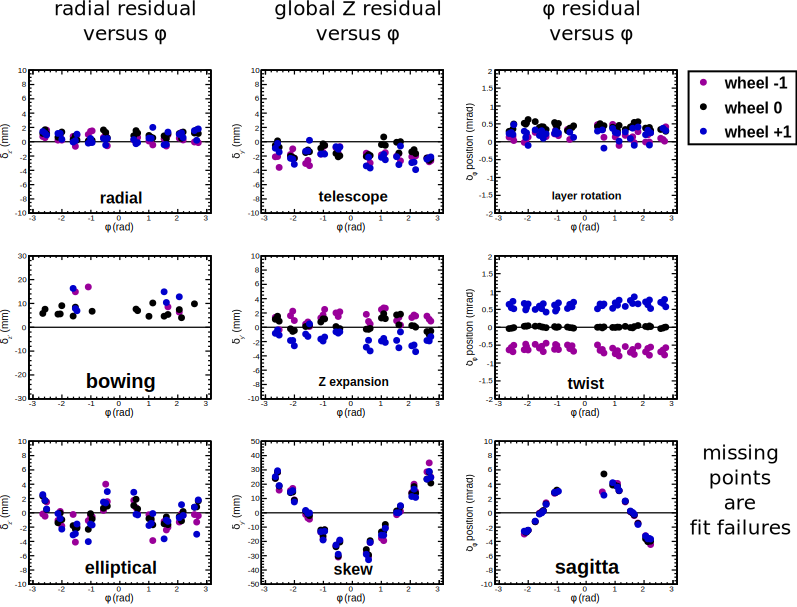
\includegraphics[height=4.9 cm]{systematics.pdf}}\hspace{-0.5 cm}}

\begin{columns}
\column{0.42\linewidth}
\centering
\textcolor{darkblue}{\scriptsize Z.~Guo, R.~Castello}
\column{0.58\linewidth}
\mbox{ }
\end{columns}
\end{frame}

\begin{frame}
\frametitle{Cosmic splitting test}
\begin{itemize}
\item ``Fractional curvature error'' $=$ {\scriptsize $\left(\frac{q}{p_T}^{\mbox{\scriptsize top}} - \frac{q}{p_T}^{\mbox{\scriptsize bottom}}\right)/\left(\sqrt{2}\frac{q}{p_T}\right)$}
\item Misalignment with 2.0~mm global distortion is correlated \mbox{with tracker,\hspace{-0.5 cm}} hence resolution is actually better than with random 0.9~mm
\item MC underestimates real resolution by 10--35\% {\scriptsize (non-alignment effects?)}
\end{itemize}

\hfill \textcolor{darkblue}{\scriptsize J.~Tucker}

\vspace{-0.5 cm}
\begin{center}
\only<1>{\includegraphics[width=0.8\linewidth]{TPFMS.png}}
\only<2>{\includegraphics[width=0.8\linewidth]{Global.png}}\mbox{\hspace{0.5 cm}}
\end{center}
\end{frame}

\begin{frame}
\frametitle{CSC alignment update}

\begin{itemize}
\item Translate/rotate CSC disks using ring-1 chambers
\item Example below: $\delta_x = 2.9$~mm, $\delta_y = 3.0$~mm, $\delta_{\phi_z} = 0.22$~mrad

$r\phi$ residuals versus $\phi$; dashed lines are chamber boundaries
\end{itemize}

\begin{columns}
\column{0.5\linewidth}
\centering

\only<1>{ME$-$1/1}\only<2>{ME$-$1/2} before

\only<1>{\includegraphics[height=\linewidth, angle=90]{demo_mem11_before.pdf}}
\only<2>{\includegraphics[height=\linewidth, angle=90]{demo_mem12_before.pdf}}
\column{0.5\linewidth}
\centering

\only<1>{ME$-$1/1}\only<2>{ME$-$1/2} after

\only<1>{\includegraphics[height=\linewidth, angle=90]{demo_mem11_after.pdf}}
\only<2>{\includegraphics[height=\linewidth, angle=90]{demo_mem12_after.pdf}}
\end{columns}

\begin{itemize}
\item Still investigating ring-2 residuals \mbox{(even-odd chambers alternate 5~mm)\hspace{-1 cm}}
\begin{itemize}
\item not reproduced at the level of RecHits in the overlap region\ldots
\end{itemize}
\end{itemize}
\end{frame}

%% \section*{First section}
%% \begin{frame}
%% \begin{center}
%% \Huge \textcolor{blue}{First section}
%% \end{center}
%% \end{frame}

\begin{frame}
\frametitle{Conclusions}
\begin{itemize}\setlength{\itemsep}{0.5 cm}
\item Reference-Target algorithm is sufficiently routine that it can
  be run under different conditions to study alignment systematics
\begin{itemize}
\item time dependence makes sense \mbox{(biggest change between CRAFTs)\hspace{-1 cm}}
\item most large changes have been identified as moved chambers
\item tracker didn't change significantly between CRAFTs to affect muon alignment
\item small effect seen in including tracker endcap
\item effect of tracker global distortions visible in MC
\end{itemize}

\item Muon system with chamber positions matched to tracker yields
  better resolution than smaller, uncorrelated errors
\begin{itemize}
\item but ideally both ought to be minimized
\end{itemize}

\item CSC bug-hunt continues, but we can produce a disk alignment even if the problem isn't found
\end{itemize}
\label{numpages}
\end{frame}

\end{document}
